\section{PROPOSED SYSTEM (METHODOLOGY)}
\label{sec:methodology}

The proposed system, \textbf{SafeSurf}, introducing an advanced phishing detection framework that combines infrastructure analysis with a machine learning ensemble. The architecture is designed for real-time inference, balancing the exhaustive depth of 111-feature analysis with the low-latency requirements of a web browser extension.

\subsection{System Architecture}
SafeSurf is organized into three major functional layers as shown in Figure \ref{fig:architecture}. The \textbf{Client Layer} (React Dashboard and Chrome Extension) handles user interaction and displays verdicts. The \textbf{Processing Layer} (FastAPI Backend) performs canonicalization, concurrency control, and feature extraction. Finally, the \textbf{Detection Layer} executes the hybrid machine learning ensemble.

\begin{figure*}[htbp]
    \centering
    \includegraphics[width=0.85\textwidth]{images/system-architecture.png}
    \caption{Layered system architecture of SafeSurf showing the interaction between the browser extension and the backend processing engine.}
    \label{fig:architecture}
\end{figure*}

\subsection{Layered Detection Pipeline}
To optimize performance, SafeSurf implements a tiered detection pipeline:
\begin{enumerate}
    \item \textbf{DNS Guard (Deterministic Gate)}: Acts as the first security layer. It performs a high-speed socket-level resolution check. If a domain results in an \texttt{NXDOMAIN} response, the request is instantly halted, preventing unnecessary computational overhead for non-existent domains.
    \item \textbf{Asynchronous Feature Extraction}: Upon passing the DNS Guard, the system extracts exactly 111 deep features across two processing tiers:
    \begin{itemize}
        \item \textbf{Layer A (Lexical)}: Evaluates URL structure, character counts, and symbol frequencies (e.g., number of dots, hyphens, and "@" symbols). These are computed locally and require practically $<1$ms.
        \item \textbf{Layer B (Infrastructure)}: Concurrently resolves DNS A/NS/MX records, SSL/TLS certificates, and WHOIS registration details using an asynchronous processing loop (\texttt{asyncio.gather}).
    \end{itemize}
    \item \textbf{Hybrid Ensemble Inference}: The extracted features are fed into a dual-engine ensemble model.
\end{enumerate}



\subsection{Hybrid Ensemble Learning Model}
The core of SafeSurf is a specialized \textbf{VotingClassifier} ensemble model \cite{ref9}, which combines infrastructure-based metrics with linguistic NLP analysis. The detection engine utilizes a weighted soft-voting algorithm that fuses the probability outputs of two distinct pipelines:
\begin{enumerate}
    \item \textbf{Infrastructure Engine (65\% weight)}: A sub-ensemble comprising Logistic Regression, LinearSVC, Random Forest, HistGradientBoosting, and Calibrated XGBoost. This engine focuses on 111-dimensional numeric vectors.
    \item \textbf{Linguistic NLP Engine (35\% weight)}: A Logistic Regression model trained on Bag-of-Words vectors generated from URL tokens (e.g., detecting keywords like "verify", "secure", or "login").
\end{enumerate}

The final ensemble probability $P_{ensemble}$ is calculated as:
\begin{equation}
    P_{ensemble} = w_{inf} \cdot P_{XGB} + w_{nlp} \cdot P_{NLP}
\end{equation}
where $w_{inf} = 0.65$ and $w_{nlp} = 0.35$. The system classifies a URL as phishing if $P_{ensemble} \geq 0.65$.

\begin{figure}[htbp]
    \centering
    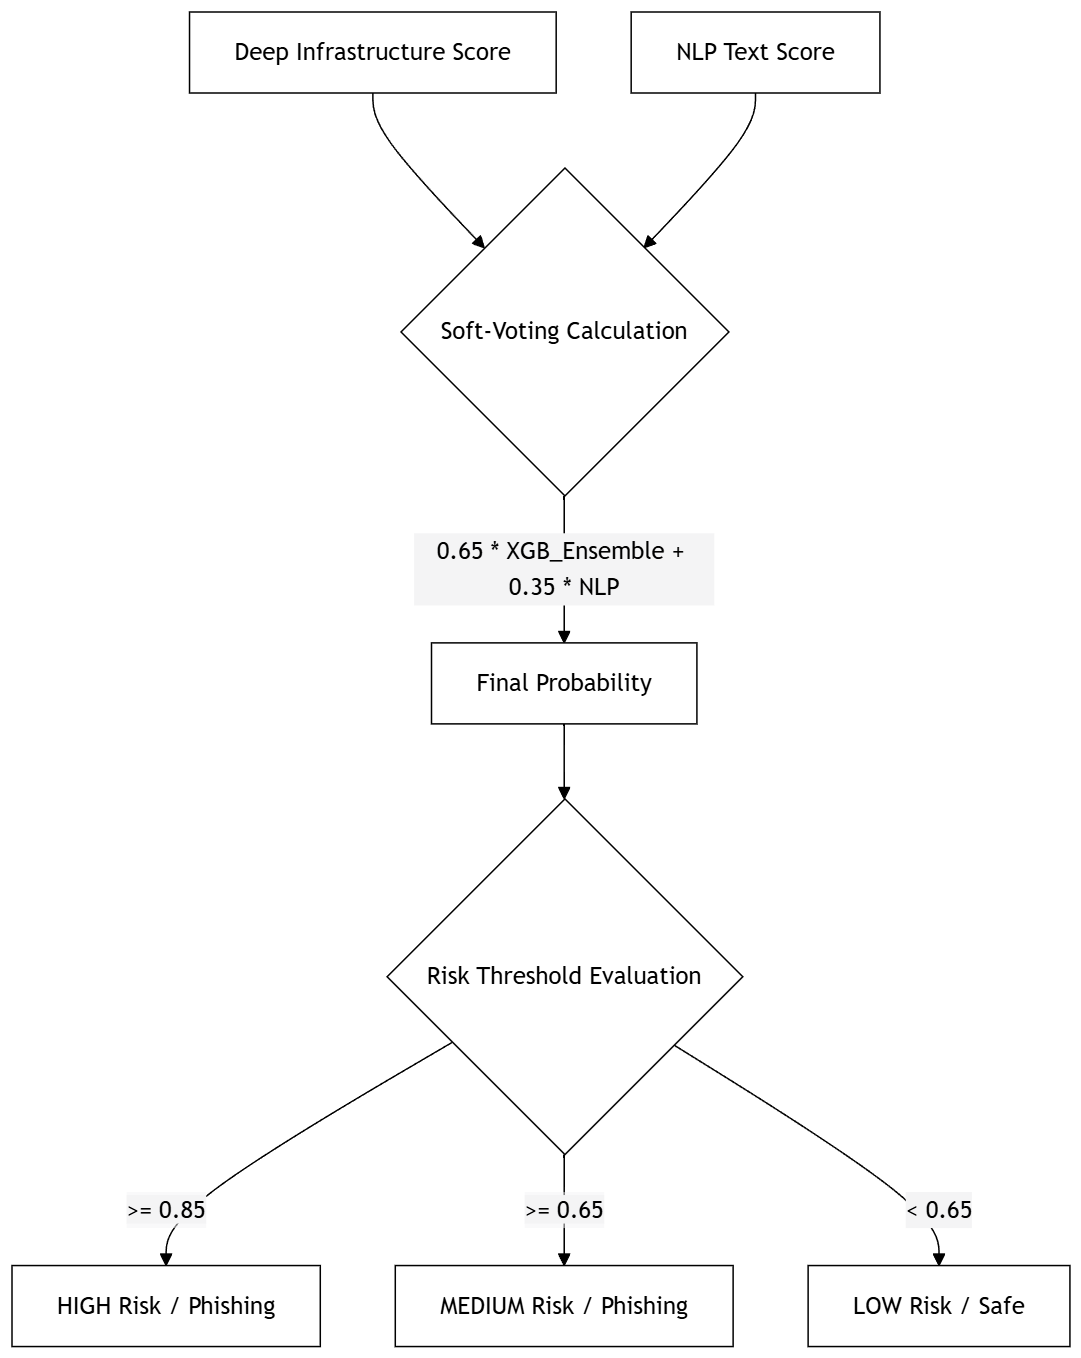
\includegraphics[width=0.9\linewidth]{images/weighted-soft-voting.png}
    \caption{Probability fusion logic of the weighted soft-voting ensemble model.}
    \label{fig:soft_voting}
\end{figure}

\subsection{Implementation \& Deployment}
The backend is developed using the high-performance \textbf{FastAPI} framework, which natively supports asynchronous operations. To ensure deployment consistency, the entire ecosystem—including the React frontend and the ML inference server—is containerized using \textbf{Docker}. A rolling 5-minute In-Memory TTL Cache (\texttt{ttl\_bucket}) is implemented to cache infrastructure results, respecting external API limits and improving performance for frequently visited domains.

\subsection{Development Workflow}
The research and development of SafeSurf followed a systematic 7-phase process to ensure the robustness of the detection engine:
\begin{figure*}[htbp]
    \centering
    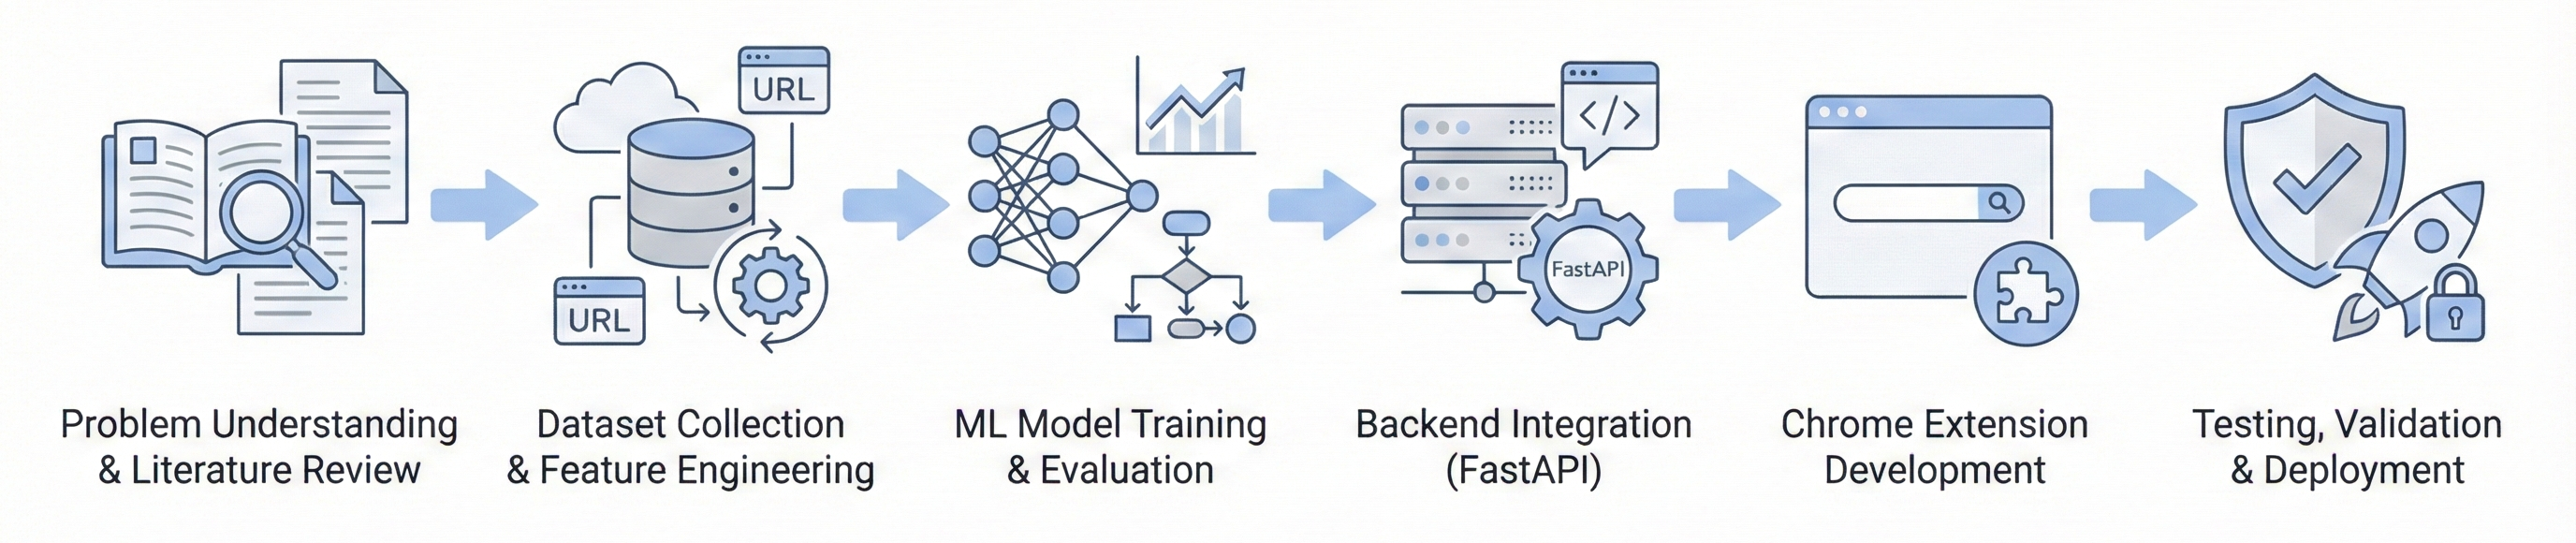
\includegraphics[width=0.85\textwidth]{images/developmemt-workflow.png}
    \caption{Overview of the 7-phase development workflow for the SafeSurf phishing detection framework.}
    \label{fig:workflow}
\end{figure*}
\begin{enumerate}
    \item \textbf{Problem Understanding}: Analyzing the limitations of current blacklist and single-model systems.
    \item \textbf{Dataset Extraction}: Massive parallel extraction from the PhiUSIIL database \cite{ref10}.
    \item \textbf{Feature Engineering}: Tokenization and 111-dimensional numeric mapping.
    \item \textbf{Model Training}: Iterative validation and hyperparameter tuning of the ensemble.
    \item \textbf{Backend Integration}: Orchestrating the soft-voting logic via FastAPI.
    \item \textbf{Client Development}: Building the React dashboard and Chrome extension.
    \item \textbf{Final Deployment}: Stress testing and containerization.
\end{enumerate}

